\clearpage{}
\section{Generalisation}
\label{inference:generalisation}

When no more types can be unified, and no more effects or type class constraints can be reduced, the graph is said to be in \emph{normal form}. We can now extract the type for $\imap$ from our graph and generalise it into a type scheme.

In DDC we refer to the complete process of building a type scheme from the information in the type graph as ``generalisation''. This process is broken down into several stages, summarised below. Note that in a concrete implementation, several of these stages can performed at the same time. For example, checking for loops through the constraints can be done while tracing them, as tracing corresponds to a simple reachability analysis.

\bigskip
\qq
\begin{tabular}{lll}
	1. & Tracing:		& isolate the type information of interest. \\
	2. & Loop checking:	& check for infinite value type errors. \\
	3. & Packing:		& pack the graphical constraints into ``flat'' form. \\
	4. & Loop breaking:	& break loops through effect and closure constraints. \\
	5. & Cleaning:		& discard non-interesting effect and closure variables. \\
	6. & Quantification:	& introduce type quantifiers. 
\end{tabular}


% ---------------------------------------------------------
\subsection{Tracing}
The first step is to trace out the section of graph that is reachable from the type variable we're interested in. For this example we're interested in $\imap$ and all equivalence classes except *0 are reachable from $s_{\imap}$. This process makes a copy of the information present in the ``global'' graph, and the operations described in the rest of this section are performed on the copy. 


% ---------------------------------------------------------
\subsection{Loop checking}
We now check for loops through the value type portion of the copied sub-graph. A classic example of a program with a looping type is:

\qq\qq
\begin{tabular}{ll}
	$x$	& $= \iCons \ x \iNil$
\end{tabular}

where $\iCons$ and $\iNil$ have the following types:

\code{
	$\iNil$	& $:: \forall r \ a. \iList \ r \ a$ \\

	$\iCons$	
		& $:: \forall r \ a \ c. \ a \to \iList \ r \ a \lfuna{c} \iList \ r \ a$ \\
		& $\rhd \ c \tme x : a$
}



After slurping and grinding constraints, this program has the following graph:
\qq\qq
\begin{tabbing}
MMMMM 	\= MM 	\= MMMMM 	\= MMMMMMMMMM 		\= MMx \= MMM \= MMM \kill
	\> \ *1	\> $\sim \quad s_x,$	\> $s_1, \ s_4, \ a_3, \ a_5$	\> \quad $=$	\> $\iList \ r_3 \ s_x$ \\
	\> \ *2	\> $\sim \quad s_2$,	\>				\> \quad $=$	\> $s_5 \lfuna{e_1 \ c_1} s_x$ \\
	\> \ *3	\> $\sim \quad s_3$,	\> $s_{\iCons}$			\> \quad $=$	\> $s_4 \lfuna{e_2 \ c_2} s_2$ \\
	\> \ *4 \> $\sim \quad s_5$,	\> 				\> \quad $=$	\> $\iList \ r_3 \ s_x$ \\
	\> \ \$1 \> $\sim \quad c_3$,	\> $c_1$			\> \quad $\tme$	\> $x : s_x$ \\
	\> \ \%1 \> $\sim \quad r_3$,	\> $r_5$ 
\end{tabbing}


The loop is through equivalence class *1. We cannot produce a flat, non-graphical type for $s_x$ because if we tried to solve its constraint our algorithm would diverge:

\code{
		& $s_x$	& $= \iList \ r_3 \ s_x$ \\
 $\equiv$	& $s_x$ & $= \iList \ r_3 \ (\iList \ r_3 \ s_x)$ \\
 $\equiv$	& $s_x$ & $= \iList \ r_3 \ (\iList \ r_3 \ (\iList \ r_3 \ s_x))$ \\
 $\equiv$	& \dots 
}

\bigskip
Unlike \cite{cardone:recursive-types} we do not attempt to handle recursive value types, so we flag them as errors instead. This is common to other compilers such as GHC, which would emit a message ``cannot construct infinite type''. Note that loops through the effect or closure portions of a type graph are \emph{not} counted as errors. We deal with these in \S\ref{Inference:Generalisation:loop-breaking}.


% ---------------------------------------------------------
\subsection{Packing}
Packing is the process of converting a set of individual type constraints into the normalised form of \ref{inference:language:normal-types}. When we pack the constraints from our $\imap$ example into this form we have:

\bigskip
\begin{tabular}{llllll}
	$s_{\imap}$	
	& \mc{3}{$= (s_x \lfuna{e_{11a} \ c_{11}} s_{11}) 
			\lfuna{e_2 \ c_1} \iList \ r_5 \ s_x 
			\lfuna{e_3 \ c_2} \ \iList \ r_6 \ s_{11}$} 
	\\[1ex]
	& $\rhd$ & $e_3$ 	& $\tme \ \iRead r_5 \lor e_6 \lor e_8$	\\
	& \ ,	 & $e_8$	& $\tme \ e_9 \lor e_{14} \lor e_{8a}$ \\
	& \ ,  	 & $e_9$	& $\tme \ e_{10} \lor e_{11} \lor e_{9a}$ \\
	& \ ,	 & $e_{11}$	& $\tme \ e_{12} \lor e_{13} \lor e_{11a}$ \\
	& \ ,	 & $e_{14}$	& $\tme \ e_{15} \lor e_{18} \lor e_3$ \\
	& \ ,	 & $e_{15}$	& $\tme \ e_{16} \lor e_{17} \lor e_{2}$ \\
	& \ , 	 & $c_{1}$	& $\tme \ \imap : (s_x \lfuna{e_{11a} \ c_{11}} s_{11}) 
							\lfuna{e_2 \ c_1} \iList \ r_5 \ s_x 
							\lfuna{e_3 \ c_2} \ \iList \ r_6 \ s_{11}$ \\
	& \ , 	 & $c_{2}$	& $\tme \  \imap : (s_x \lfuna{e_{11a} \ c_{11}} s_{11}) 
							\lfuna{e_2 \ c_1} \iList \ r_5 \ s_x 
							\lfuna{e_3 \ c_2} \ \iList \ r_6 \ s_{11}$ \\
	&	&		& $\ \ \ \ \ \ \ \lor \ f : s_x \lfuna{e_{11a} \ c_{11}} s_{11}$
\end{tabular}

\bigskip
Although the body of this type is now in the familiar form, there is still a hash of effect and closure constraints. However, notice that there is only one use each of the variables $e_8, \ e_9, \ e_{11}, \ e_{14}$ and $e_{15}$, and they are not mentioned in the body of this type. From a compiler optimisation point of view, the only effect information that we need to preserve is the manifest effect of each function arrow. The fact that, say, $e_3$ includes $e_8$ and $e_8$ includes $e_9$ does not matter, as long as all of the appropriate variables are reachable from $e_3$.

This means that we can inline the constraints on $e_8$, $e_9$ and so on into the constraint for $e_3$. We can also use the closure trimming process discussed in \S\ref{System:Closure:trimming} to simplify the constraints for $c_1$ and $c_2$. This produces:

\bigskip
\code{	
	$s_{\imap}$	
	& \mc{3}{$= (s_x \lfuna{e_{11a} \ c_{11}} s_{11}) 
			\lfuna{e_2 \ c_1} \iList \ r_5 \ s_x 
			\lfuna{e_3 \ c_2} \ \iList \ r_6 \ s_{11}$} 
	\\[1ex]
	& $\rhd$ & $e_3$ 	& $\tme \ \iRead r_5 \lor e_6 \lor e_8 \lor e_9 \lor e_{14} \lor e_{8a}$ \\
	&	 &		& $ \qq \qq \ \ \ \lor \ e_{10} \lor e_{11} \lor e_{9a} 
					\lor e_{12} \lor e_{13} \lor e_{11a}$ \\
	&	 &		& $ \qq \qq \ \ \ \lor \ e_{15} \lor e_{18} \lor e_3 
					\lor e_{16} \lor e_{17} \lor e_{2}$ \\
	& \ , 	 & $c_{1}$	& $\tme \ \imap  : c_1$ \\
	& \ , 	 & $c_{2}$	& $\tme \  \imap : c_1 \lor \ f : c_{11}$
}


% ---------------------------------------------------------
\subsection{Loop breaking}
\label{Inference:Generalisation:loop-breaking}
As discussed in \S\ref{System:Effects:recursive}, we can use the lattice structure of effects and closures to break loops through effect and closure constraints. If the type of a particular value variable contains looping constraints, then breaking these loops makes the type simpler, and allows it to be exported to the core language. The following diagram shows a loop through the effect portion of the type for $\imap$, as it was after the first stage of packing:

\begin{center}
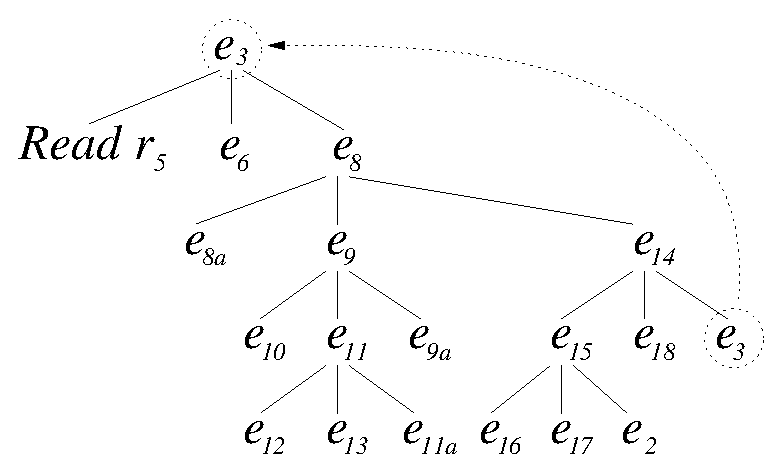
\includegraphics[scale=0.5]{3-Inference/fig/generalisation/loop-effect}
\end{center}

Notice how the structure of this effect graph echos the original abstract syntax tree for $\imap$. In the effect graph we can see two branches, headed by $e_9$ and $e_{14}$, corresponding to the two alternatives of the original case expression. We can also see the recursive call via $e_3$. $\imap$ applies itself, so the effect of $\imap$ includes the effect of $\imap$. Similarly, $\imap$ references itself, so the closure of $\imap$ includes the closure of $\imap$.

However, although recursion in the function's \emph{definition} serves a useful purpose, the fact that its effect and closure is also recursive is not exploited by our analysis. We need to retain the set of effects caused by an application of $\imap$, that is, the effects reachable from $e_3$, but this information would not be lost if we substituted $\bot$ for its recursive occurrence. Finally, the constraints $e_3 \tme e_3$ and $c_1 \tme \imap : c_1$ are trivially satisfied, so can be discarded. This leaves us with:

\bigskip
\qq
\begin{tabular}{llll}
	$s_{\imap}$	
		& \mc{3}{$= (s_x \lfuna{e_{11a} \ c_{11}} s_{11}) 
				\lfuna{e_2 \ c_1} \iList \ r_5 \ s_x 
				\lfuna{e_3 \ c_2} \ \iList \ r_6 \ s_{11}$} 
		\\[1ex]
		& $\rhd$ & $e_3$ 	& $\tme \ \iRead r_5 \lor e_6 \lor e_8 \lor e_9 \lor e_{14} \lor e_{8a}$ \\
		&	 &		& $ \qq \qq \ \ \ \lor \ e_{10} \lor e_{11} \lor e_{9a} \lor e_{12} \lor e_{13} \lor e_{11a}$ \\
		&	 &		& $ \qq \qq \ \ \ \lor \ e_{15} \lor e_{18} \lor \bot \lor e_{16} \lor e_{17} \lor e_{2}$ \\
		& \ , 	 & $c_{2}$	& $\tme \  \imap : c_1 \lor \ f : c_{11}$
\end{tabular}


% ---------------------------------------------------------
\subsection{Cleaning}
There are still a large number of effect and closure variables in our type that don't provide any useful information. For example, $e_6$ is the effect of evaluating the variable $\iNil$, but evaluating a variable doesn't have a visible effect. Also consider $e_9$, the effect of evaluating $\iCons \ (f \ x)$. The evaluation of $(f \ x)$ itself has the effect $e_{11}$, which is interesting because it depends on the function argument passed to map, but the partial application of $\iCons$ to the result does not have an effect, so is boring. In any event, the constraint on $e_3$ already contains $e_{11}$, so it doesn't need to include $e_9$ as well.

We define boring effect and closure variables to be the ones that are completely unconstrained. Such variables are not mentioned in the type environment, in a parameter of the type being generalised, or on the left of an (in)equality. If a variable is in the type environment then it depends on a definition in a higher scope of the program. In this case, a more interesting type may be unified into the variable later in the inference process. If it is mentioned in a parameter type then it may be different for each application of the function. If it is on the left of an (in)equality then it depends on other types. For our example, $e_{11a}, \ c_{11}, \ e_{3}$ and $c_{2}$ are interesting, and the rest are boring. We substitute $\bot$ for boring variables, then use the definition of $\lor$: 

\bigskip
\qq
\begin{tabular}{llll}
	$s_{\imap}$	
		& \mc{3}{$= (s_x \lfuna{e_{11a} \ c_{11}} s_{11}) 
				\lfun \iList \ r_5 \ s_x 
				\lfuna{e_3 \ c_2} \ \iList \ r_6 \ s_{11}$} 
		\\[1ex]
		& $\rhd$ & $e_3$ 	& $\tme \ \iRead r_5 \lor e_{11a}$ \\
		& \ , 	 & $c_{2}$	& $\tme \ f : c_{11}$
\end{tabular}


% ---------------------------------------------------------
\subsection{Quantification}
We can now add quantifiers to our type and create a type scheme. There are several restrictions as to what variables can be quantified, which we will recall in a moment, but for this example none apply. After quantification we have:

\bigskip
\qq
\begin{tabular}{llll}
	$s_{\imap}$	
		& \mc{3}{$= \forall s_x \ s_{11} \ r_5 \ r_6 \ e_{11a} \ c_{11} \ e_3 \ c_2$} \\[1ex]
		& \mc{3}{$. \ \ \ \ (s_x \lfuna{e_{11a} \ c_{11}} s_{11})
				\lfun \iList \ r_5 \ s_x \lfuna{e_3 \ c_2} \ \iList \ r_6 \ s_{11}$} 
		\\[1ex]
		& $\rhd$ & $e_3$ 	& $\tme \ \iRead \ r_5 \lor e_{11a}$ \\
		& , 	 & $c_{2}$	& $\tme \ f : c_{11}$
\end{tabular}

\bigskip
We will also rewrite the quantified variables to use more familiar names:

\qq
\begin{tabular}{llll}
	$s_{\imap}$	
		& \mc{3}{$= \forall a \ b \ r_1 \ r_2 \ e_1 \ e_2 \ c_1 \ c_2$} \\[1ex]
		& \mc{3}{$. \ \ \ \ (a \lfuna{e_1 \ c_1} b)
				\lfun \iList \ r_1 \ a  \lfuna{e_2 \ c_2} \ \iList \ r_2 \ b$} 
		\\[1ex]
		& $\rhd$ & $e_2$ 	& $\tme \ \iRead \ r_1 \lor e_{1}$ \\
		& , 	 & $c_2$	& $\tme \ f : c_{1}$
\end{tabular}

\medskip
At this stage we could also apply the the effect masking rules from \S\ref{System:Effects:masking} and \S\ref{System:Closure:masking}, though none apply in this example. Once generalisation is complete we update the $s_{\imap}$ equivalence class in the global graph so it contains this new type scheme.

\subsubsection{The non-generalisable variables}
There are several reasons why a particular type variable may not be permitted to be generalised. All but the first were discussed in the previous chapter.

Don't generalise:
\begin{enumerate}
\item	Variables free in the type environment. This is the standard restriction for Hindley-Milner
	type systems \cite{milner:type-polymorphism, damas:principle-type-schemes}. However, as we're
	performing type inference instead of type \emph{checking}, the real type environment is not
	close at hand. We instead use the method discussed in \S\ref{inference:ordering} to
	determine the value variables that are free in the binding whose type is being generalised.
	The types of these variables can be determined from the graph, and we hold their free type
	variables monomorphic. This achieves the same result.
	
\item	Dangerous type variables, which were discussed in \S\ref{System:Closure:dangerous} and 
	\S\ref{Inference:Language:dangerous-variables}. These are variables that appear free under
	type constructors whose regions are constrained to be mutable. Dangerous type variables must be
	held monomorphic to avoid the problem with polymorphic update that was discussed in \S\ref{System:Update}.

\item	Material region variables, which were discussed in \S\ref{System:Closure:non-material-regions}.
	Material regions correspond with objects that are shared between all uses of the variable
	whose type is being generalised. These must also be held monomorphic.
\end{enumerate}


% ---------------------------------------------------------
\subsection{Late constraints and post-inference checking}
\label{Inference:Generalisation:late-constraints}

The fact that mutability constraints influence what type variables are quantified introduces a slight complication into the inference process. The type inferencer might quantify a type variable while assuming that a particular region is constant, but later discover a mutability constraint that indicates it shouldn't have quantified. We refer to such mutability constraints as \emph{late} constraints. The following example demonstrates the problem:

\bigskip
\code{	\mc{2}{$\ilateFun \ ()$} \\
	\ $= \kdo$ 	& $\iref$	& $ = \inewRef \ \iid$		\\
			& $f$		& $ = \lambda(). \ireadRef \ \iref$ \\
			& \mc{2}{$\iwriteRef \ \iref  \ \isucc$}	\\
	 		& \mc{2}{$f \ ()$ \ ``\texttt{oh noes}''}
}

with

\code{	$\iid$ 	
		& $::$	& $\forall a. \ a \to a$ 	
	\\[1ex]
	$\isucc$
		& $::$		& $\forall r_1 \ r_2 \ e_1. \ \iInt \ r_1 \lfuna{e_1} \iInt \ r_2$	 \\
		& $\rhd$	& $e_1 \tme \iRead \ r_1$
	\\[1ex]
	$\inewRef$
		& $::$		& $\forall a \ r_1. \ a \to \iRef \ r_1 \ a$
	\\[1ex]
	$\ireadRef$
		& $::$		& $\forall a \ r_1 \ e_1. \iRef \ r_1 \ a \lfuna{e_1} a$ \\
		& $\rhd$	& $e_1 \tme \iRead \ r_1$
	\\[1ex]
	$\iwriteRef$
		& $::$		& $\forall a \ r_1 \ e_1 \ c_1. \iRef \ r_1 \ a \to a \lfuna{e_1 \ c_1} ()$ \\
		& $\rhd$	& $e_1 \tme \iWrite \ r_1$ \\
		& ,		& $c_1 \tme x : \iRef \ r_1 \ a$ \\
		& ,		& \mc{2}{$\iMutable \ r_1$}
}

From the types of $\inewRef$, $\ireadRef$ and $\iwriteRef$, we see that an object of type $\iRef \ r_1 \ a$ is only treated as mutable if we actually apply the $\iwriteRef$ function to it. If we only ever \emph{read} a reference, then there is no need to mark it as mutable or restrict the type of the contained value. However, with our $\ilateFun$ example, the type inferencer will only discover that $\iref$ is mutable when it processes the third line of the do-expression. If it considers the bindings in-order, and generalises the type of $\iref$ while assuming constancy, it will get:

\code{
	$\iref :: \forall a. \iRef \ r_1 \ (a \to a)$
}

\clearpage{}

with this scheme, the type of $f$ becomes:

\code{
	$f$	& $::$ 		& $ \forall b \ e_1 \ c_1. \ () \lfuna{e_1 \ c_1} b \to b$ \\
		& $\rhd$	& $e_1 \tme \iRead \ r_1$ \\
		& ,		& $c_1 \tme \iref : \iRef \ r_1 \ (b \to b)$
}

Later, the inferencer will discover the call to $\iwriteRef$, which places a mutability constraint on $r_1$ and invalidates the previous type scheme for $\iref$. Note that it is not safe to simply change the scheme for $\iref$ to a less general one ``on the fly'', because the old scheme was instantiated when inferring the type of $f$, and now that type is wrong as well. 

A simple solution is to wait until type inference is complete, re-generalise the types of all let-bound variables, and compare the resulting type schemes against the previously inferred ones. Waiting until inference is complete ensures that all the available mutability constraints have made their way into the type graph. If a newly generalised scheme is different to its original version, then a mutability constraint must have been added to the graph after the original was created. This is reported as an error.

This solution has the disadvantage of requiring the types of polymorphic mutable objects to be given explicitly as signatures. For example, although the following program will not cause a problem at runtime, it will be marked as erroneous:

\code{
	$\ifalseLate$ \\	
	\ $= \kdo$ 	& $\iref$	& $ = \inewRef \ \iid$		\\
			& \mc{2}{$\iwriteRef \ \iref  \ \isucc$}	\\
			& \mc{2}{$(\ireadRef \iref) \ 5$}
}

Adding a type signature ensures that the inferencer will treat $\iref$ as being mutable when its type is generalised:

\code{
	$\ifixedLate'$ \\
	\ $= \kdo$ 	& \mc{2}{$\iref :: \iRef \ r_1 \ (a \to a) \rhd \iMutable \ r_1$} \\
			& $\iref$	& $ = \inewRef \ \iid$		\\
			& \mc{2}{$\iwriteRef \ \iref  \ \isucc$}	\\
			& \mc{2}{$(\ireadRef \iref) \ 5$}
}

\bigskip
An alternate solution would be to re-generalise the type of $\iref$ at each instantiation point. If the newly generalised scheme was different to the previous one, then we could backtrack to original definition and re-type the subsequent program using the new scheme. We could also perform backtracking in a coarse grained manner, by doing the post-inference check as before, but re-typing the \emph{whole} program if any schemes were different. However, backtracking adds extra complexity, and we expect programs like the above to be rare, so we use the simpler non-backtracking solution in our implementation.

The BitC compiler also checks for the late constraint problem \cite{sridhar:type-inference-systems-language}. It does not backtrack, but performs the check during type inference proper. It also uses local heuristics to guess whether a particular variable is mutable, without performing complete inference. Before generalising the type of a variable it inspects how it is used later in the function. If the variable is updated locally, its type is generalised using this information. This is possible in BitC because the assignment operator $:=$ is baked into the language, instead of being defined in the standard libraries.

